\section{Presentazione del caso di studio}
Il sistema oggetto dell'analisi in questione eroga le seguenti tipologie di servizi:
\begin{enumerate}
\item \textbf{Unica Operazione} (e.g. ricarica \textsl{PostePay}, invio raccomandata e pagamento di massimo 3 bollettini)
\item \textbf{Pagamenti \& Prelievi} (e.g. pagamento di un numero arbitrario di bollettini, bollo auto e libretti)  
\item \textbf{Spedizioni \& Ritiri} (e.g. invio corrispondenza, lettere, pacchi e raccomandate)
\end{enumerate}

Per essere serviti i clienti possono:
\begin{itemize}
\item Recarsi all'ufficio postale, prendere un ticket relativo al servizio a cui sono interessati e mettersi in coda in attesa del proprio turno. Nel caso in cui essi dimostrano di essere titolari di un conto \textsl{BancoPosta} potranno accodarsi in una fila dedicata.
\item Prenotare un ticket mediante l'applicazione \textsl{"Ufficio Postale"} per una determinata fascia oraria, al fine di essere serviti dal primo sportello disponibile entro 40 minuti, ma non prima, dall'orario di prenotazione.
\end{itemize}

Un insieme di sportelli serve le richieste degli utenti in accordo alle seguenti regole: 
\begin{enumerate}[label=R\arabic*)]
\item I clienti titolari di un conto \textsl{BancoPosta} vengono serviti con una priorità maggiore rispetto agli altri, indipendentemente dal ticket scelto.
\item Poiché, per definizione, ticket di tipo \textbf{Unica Operazione} dovrebbero richiedere meno tempo per essere processati, viene assegnata loro la massima priorità
\item I ticket di tipo \textbf{Spedizioni \& Ritiri} vengono serviti da uno sportello dedicato il quale, in assenza di questa tipologia di ticket, opera come gli altri. Il comportamento di tale servente è schematizzato in figura \ref{fig:presentazione-1}. 
\end{enumerate}

\begin{figure}[ht]
\centering
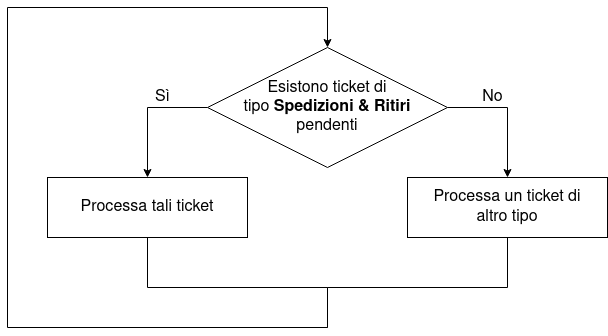
\includegraphics[width=0.75\linewidth]{presentazione-1}
\scaption{Schema del comportamento del servente dedicato ai ticket di tipo \textbf{Spedizioni \& Ritiri}}
\label{fig:presentazione-1}
\end{figure}